\documentclass[12pt]{article}
\usepackage[top=1in, bottom=1in, left=.75in, right=.75in]{geometry}
\usepackage{amsmath}
\usepackage{fancyhdr}
\usepackage{graphicx}
\usepackage{txfonts}
\usepackage{multicol}
\usepackage{wrapfig}
\usepackage[scaled=0.86]{helvet}
\usepackage{anyfontsize}
% \usepackage{times}
% \usepackage[lf]{MinionPro}
\usepackage{tikz,pgfplots}

\usepackage{textcomp,enumerate}

\renewcommand{\emph}[1]{\textsf{\textbf{#1}}}

\def\degC{{}^\circ{\rm C}}
\def\ra{\rightarrow}

\newcommand{\blank}[1]{\rule{#1}{0.75pt}}

% \setmainfont{Times}
% \def\sansfont{Lucida Grande Bold}
\parindent 0pt
\parskip 4pt
\pagestyle{fancy}
\fancyfoot[C]{\emph{\thepage}}
\fancyhead[L]{\ifnum \value{page} > 1\relax\emph{Math 251: Final Exam}\fi}
\fancyhead[R]{\ifnum \value{page} > 1\relax\emph{December 7, 2021}\fi}
\headheight 15pt
\renewcommand{\headrulewidth}{0pt}
\renewcommand{\footrulewidth}{0pt}
\let\ds\displaystyle
\def\continued{{\emph {Continued....}}}
\def\continuing{{\emph {Problem \arabic{probcount} continued....}}\par\vskip 4pt}


\newcounter{probcount}
\newcounter{subprobcount}
\newcommand{\thesubproblem}{\emph{\alph{subprobcount}.}}
\def\problem#1{\setcounter{subprobcount}{0}%
\addtocounter{probcount}{1}{\emph{\arabic{probcount}.\hskip 1em(#1)}}\par}
\def\subproblem#1{\par\hangindent=1em\hangafter=0{%
\addtocounter{subprobcount}{1}\thesubproblem\emph{#1}\hskip 1em}}
\def\probskip{\vskip 10pt}
\def\medprobskip{\vskip 2in}
\def\subprobskip{\vskip 45pt}
\def\bigprobskip{\vskip 4in}

\begin{document}
{\emph{\fontsize{26}{28}\selectfont Math F251\hfill
{\fontsize{32}{36}\selectfont Final Exam}
\hfill Fall 2021}}
\vskip 0.5cm
\strut\vtop{\halign{\emph#\hskip 0.5em\hfil&#\hbox to 2in{\hrulefill}\cr
\emph{\fontsize{18}{22}\selectfont Name:}&\cr}}
\hfill
\vtop{\halign{\emph{\fontsize{18}{22}\selectfont #}\hfil& \emph{\fontsize{18}{22}\selectfont\hskip 0.5ex $\square$ #}\hfil\cr
Section: & F01 (Faudree)\cr
\noalign{\vskip 4pt}
         & F02 (Gossell)\cr
\noalign{\vskip 4pt}
         & UX1 (Gossell)\cr}}

{\fontsize{18}{22}\selectfont\emph{Rules:}}

You have 2 hours to complete the exam.  

Partial credit will be awarded, but you must show your work.

No other aids are permitted.

Place a box around your  \fbox{FINAL ANSWER} to each question where appropriate.

Turn off anything that might go beep during the exam.
\vskip 0.5cm


\begin{center}
{
\sf\fontsize{16pt}{22pt}\selectfont
\renewcommand{\arraystretch}{0.8}
\begin{tabular}{|c|c|c|}
\hline
Problem & Possible & Score \\ \hline
1 & 10 & \\ \hline
2 & 8 & \\ \hline
3 & 8 & \\ \hline
4 & 8 & \\ \hline
5 & 10 & \\ \hline
6 & 10 & \\ \hline
7 & 6 & \\ \hline
8 & 6 & \\ \hline
9 & 5 & \\ \hline
10 & 5 & \\ \hline
11 & 12 & \\ \hline
12 & 12 & \\ \hline
Extra Credit& 5 & \\ \hline
Total & 100 & \\ \hline
\end{tabular}
}
\end{center}

\vfill
\newpage
\problem{10 points} Evaluate the following limits. If you use L'Hopital's Rule, please indicate the form of the limit ($0/0$ or $\infty/\infty$).\\


\subproblem{} $\displaystyle \lim_{x \rightarrow 4} \frac{\frac{1}{4}-\frac{1}{x}}{x-16}.$

\vfill
\subproblem{} $\displaystyle \lim_{x \rightarrow 3^-} \frac{4x^2-3x}{x^2-7x+12}$
%\item $\lim_{x \rightarrow \infty} \frac{(x-2)(x-3)}{4x^2+\sqrt{x}}$

\vfill
\problem{8 points} Find the derivative of each of the following functions. You do not need to simplify your answer.\\
\subproblem{} $\displaystyle f(x) = (\sin x)( \ln(x^3 + 1))$\\

$f'(x)=$\\
\vfill
\subproblem{}  $\displaystyle g(x) = e^{\sqrt{x}}+3x^6+\cos\left(\frac{\pi}{4}\right)$\\

$g'(x)=$\\

\vfill

\newpage

\problem{8 points} Evaluate the following indefinite integrals.\\
\subproblem{} $\displaystyle \int \left(4x^2-\frac{2}{x^4}\right) dx$

\vfill
\subproblem{} $\displaystyle \int \frac{\sec^2 x}{\tan x} dx$

\vfill


\problem{8 points} The temperature in a cabin is given by
\[
T(t)= 50+\frac{15t}{t+1}
\]
where $T$ is measured in degrees Fahrenheit and 
$t\ge 0$ is measured in minutes after starting the wood stove. 

\subproblem{} At what \textbf{rate} is the temperature changing at time $t=0$? Include units in your answer.

\vfill
\subproblem{} Compute $\lim_{t\to\infty} T(t)$ and explain
what this number means in language the general public might understand.

\vfill

\newpage

\problem{10 points} A drone is launched off a 2-foot platform. Its upward velocity in feet per second at $t$ seconds is measured by the function $v(t)=\frac{5}{1+t^2}$. 


\subproblem{} Find $h(t)$, the height of the drone at $t$ seconds.

\vfill

\subproblem{}  Find $h(1)$, the height after $1$ second. Include units. Hint: $\tan (\pi/4) =1.$


\vskip 2cm


\subproblem{}  Find $a(t)$, the acceleration function at $t$ seconds. 

\vfill

\subproblem{}  Find $a(1)$, the acceleration after $1$ second. Include units.

\vskip 2cm


\subproblem{}  Find $v(1)$, the upward velocity after $1$ second. Include units.

\vskip 2cm

\subproblem{}  Use your answers from parts (d) and (e) above to determine whether the drone speeding up or slowing down when $t=1.$
\vfill
\newpage

\problem{10 points} A manufacturer discovers that the revenue gained by producing and selling $x$ products is $R(x)=960x$ and the cost is $C(x)=3x^2+5000$.
\subproblem{}   Write the profit function, $P(x)$. (Hint: Remember that profit is revenue minus cost: $P(x)=R(x)-C(x).$)
\vspace{.8in}
\subproblem{}   What is the domain of the profit function?
\vspace{.8in}
\subproblem{}   How many products should the manufacturer produce to maximize the profit? Be sure to justify that your answer is correct. That is, use Calculus to show that your answer indeed does represent a maximum or minimum.
\vfill

\problem{6 points} The volume of a spherical balloon is given by $V=\frac{4}{3}\pi r^3$. If the balloon is being inflated at a rate of $32\pi$ cubic inches per minute, how fast is the balloon's radius changing when the radius is $2$ inches? Give units with your answer.
\vfill

%\problem{10 points}  Find the equation of the line tangent to $f(x)= 5 + \ln(2\sin x - 3\cos x + 4)$ at the point $(0,5)$.
\newpage

\problem{6 points}  
The function $G(x)$ is continuous on its domain $(-\infty,0) \cup (0,\infty).$
\begin{itemize}
\item $G'(x)$ is positive for all x in the domain  $(-\infty,0) \cup (0,\infty).$
\item $G''(x)$ is negative in the interval $(0,2)$
\item $G''(x)$ is positive in the interval $(-\infty,0) \cup (2, \infty).$
\item $\displaystyle\lim_{x\to-\infty} G(x)=-1$.
\item $\displaystyle\lim_{x\to 0^+} G(x)=-\infty$ and $\displaystyle\lim_{x\to 0^-} G(x)=\infty$
\end{itemize}
Sketch the graph of $G(x)$.  
\vfill
\begin{center}
\begin{tikzpicture}[scale=1]
\draw[->] (-6.2,0) -- (6.2,0) node[right] {$x$};
\draw[->] (0,-6.2) -- (0,6.2) node[left] {$y$};
\draw[help lines, dashed] (-6.2,-6.2) grid (6.2,6.2);
\end{tikzpicture}
\end{center}

\vfill

\newpage

\problem{5 points} Consider the function $Q(x)$ graphed below. 

\begin{center}
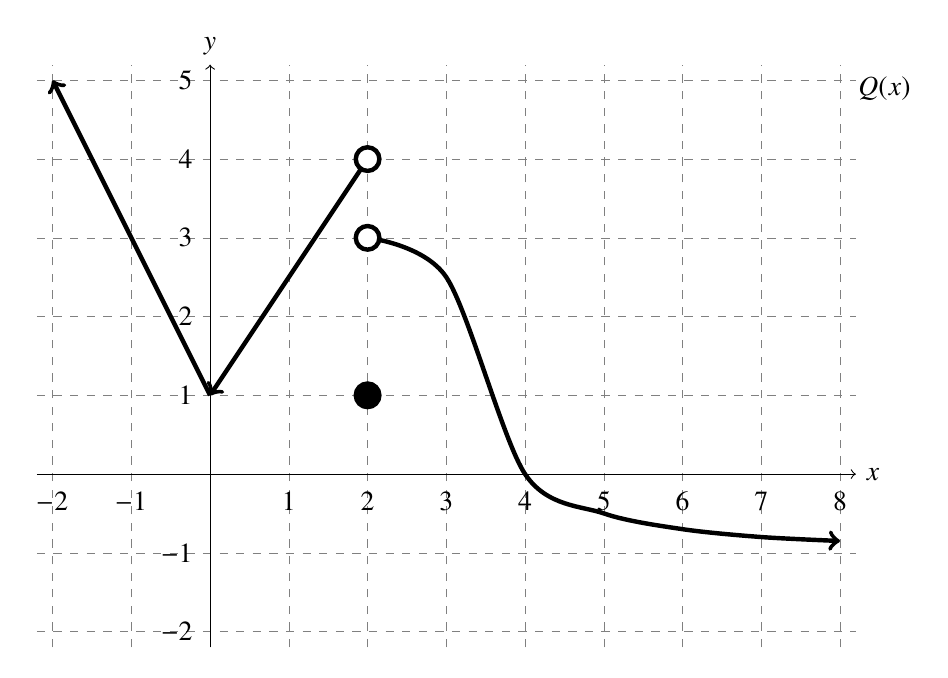
\begin{tikzpicture}[scale=1]
\draw[help lines, dashed] (-2.2,-2.2) grid (8.2,5.2);
\draw[->] (-2.2,0) -- (8.2,0) node[right] {$x$};
\draw[->] (0,-2.2) -- (0,5.2) node[above] {$y$};
\draw  (8.1,4.9) node[right] {$Q(x)$};
\draw[ultra thick, <-] plot coordinates {(-2,5) (0,1)};
\draw[ultra thick, <-] plot coordinates {(0,1) (2,4)}; 
\draw[ultra thick, ->] plot [smooth] coordinates {(2,3) (3,2.5) (4,0) (5,-0.5) (6,-0.7) (7,-0.8) (8,-0.85) };
\node[shape=circle, ultra thick, inner sep=1pt, draw,fill=white,minimum size=3mm] at (2,4){};
\node[shape=circle, ultra thick, inner sep=1pt, draw,fill=white,minimum size=3mm] at (2,3){};
\node[shape=circle, ultra thick, inner sep=1pt, draw,fill=black,minimum size=3mm] at (2,1){};

%\draw[style= ultra thick] (1,0) arc (0:180:1);
%\draw[style=ultra thick] (1,0) --(4,-1)--(5,0);
\foreach \x in {-2,-1,1,2,3,4,5,6,7,8}
\draw (\x,-0.1) node[below] {$\x$};
\foreach \y in {-2,-1,1,2,3,4,5}
\draw (-0.1,\y) node[left] {$\y$};
%\node[shape=circle, ultra thick, inner sep=1pt, draw,fill=white,minimum size=3mm] at (0,3){};
\end{tikzpicture}
\end{center}

\bigskip
\subproblem{} Find $\displaystyle \lim_{x \to 2^-} Q(x)$
\vskip 0.75cm

\subproblem{} Find $\displaystyle \lim_{x \to 4} Q(x)$
\vskip 0.75cm

\subproblem{} Find $\displaystyle \lim_{x \to \infty} Q(x)$
\vskip 0.75cm

\subproblem{} For what values of $x$, if any, does $Q(x)$ fail to be continuous?
\vfill

\subproblem{} At what values of $x$, if any, does $Q'(x)$ not exist?
\vfill

\newpage
\problem{5 points} Consider the function $f(x)$ graphed below. 

\begin{center}
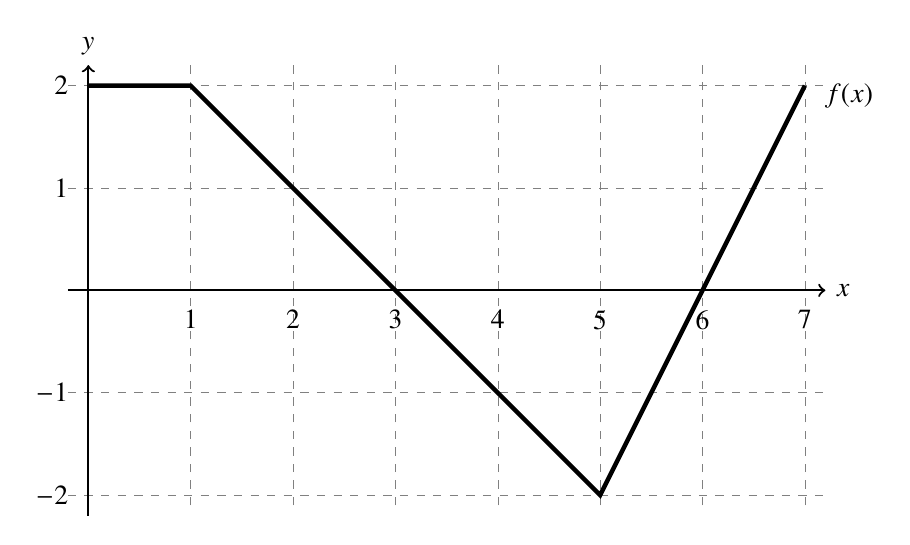
\begin{tikzpicture}[scale=1.3]
\draw[help lines, dashed] (-0.2,-2.1) grid (7.2,2.2);
\draw[thick,->] (-0.2,0) -- (7.2,0) node[right] {$x$};
\draw[thick,->] (0,-2.2) -- (0,2.2) node[above] {$y$};
\draw  (7.1,1.9) node[right] {$f(x)$};
%\node at (-.1,-.15){$0$};
\draw[style= ultra thick] (0,2) --  (1,2)--(5,-2)--(7,2);
%\draw[style= ultra thick] (1,0) arc (0:180:1);
%\draw[style=ultra thick] (1,0) --(4,-1)--(5,0);
\foreach \x in {1,2,3,4,5,6,7}
\draw (\x,-0.1) node[below] {$\x$};
\foreach \y in {-2,-1,1,2}
\draw (-0.1,\y) node[left] {$\y$};
\end{tikzpicture}
\end{center}

\bigskip
\subproblem{} What is the value of $f(6)$?
\vskip 0.75cm

\subproblem{} What is the value of $f'(6)$?
\vskip 0.75cm

%\subproblem{} What is the value of $\ds \int_{0}^7 f(x)\;dx$?
%\vfill

%\subproblem{} At what values of $x$, if any, does $f'(x)$ not exist?
%\vfill

The following questions concern $H(x) = \int_0^x f(s)\;ds$.
\bigskip

\subproblem{} What is the value of $H(7)$?
\vfill

\subproblem{} What is the value of $H'(2)$?
\vfill
\subproblem{} At what values of $x$ does $H(x)$ have a local minimum?
\vfill

\newpage
\problem{12 points} The following questions concern $\displaystyle f(x)=\frac{x^2-1}{(x-3)^2}.$ Note $\displaystyle f'(x)=-\frac{2(3x-1)}{(x-3)^3}$ and $\displaystyle f''(x)=\frac{12(x+1)}{(x-3)^4}.$
\subproblem{} Find any critical points of $f(x).$
\vspace{1in}
\subproblem{} Identify the locations of any local minimums or local maximums. Justify your conclusions. If no local minimum or local maximum exists, state this explicitly.
\vfill
\subproblem{} Does $f(x)$ have any inflection points? Justify your conclusions.
\vfill
\newpage

\problem{12 points}
Water flows into a tank at a rate of $r(t)=10+4t-t^2$ liters per minute from $t=0$ to $t=5$ minutes.

%\subproblem{} Compute $r(0)$ and $r(2)$. Then
%explain what these numbers mean in language the general public would understand.
%\vfill

\subproblem{}  Compute $\displaystyle \int_0^2 r(t) \: dt.$
\vfill

\subproblem{} Interpret your answer from part (a) in the context of the problem. Make sure to include units.
\vspace{1.3in}

\subproblem{}  At time $t=0$, the tank contained 40 liters of water.  How much water is in the tank at time $t=2$?
\vspace{.8in}
%\subproblem{} At what time is the rate of flow of the water maximized?
%\vfill

%\problem{10 points} Recall that the definition of the derivative of the function $f(x)$ is given by 
%
%$$ f'(x)=\lim_{h \to 0} \frac{f(x+h)-f(x)}{h}.$$
%
%Use this definition to find the derivative of $f(x)=5x-x^2.$
%
%
%
%
%\newpage

\problem{Extra Credit: 5 points} Evaluate $\displaystyle\lim_{x \rightarrow 0^+} \tan x \ln x$. You must show your work.
\vfill
\end{document}
